\documentclass[11pt]{article}
\usepackage[margin=0.60in, paperwidth=8.5in, paperheight=11in]{geometry}
\usepackage{amsfonts}
\usepackage{amsmath}
\usepackage{amssymb}
\usepackage{bm}
\usepackage{authblk}
\usepackage{graphicx}
\usepackage{listings}
\usepackage{array}
\usepackage{booktabs}
\usepackage{titlesec}
\usepackage{pgfplotstable}

\newcommand{\bs}[1]{\boldsymbol{#1}}
\newcommand{\del}[2]{\frac{\partial {#1}}{\partial {#2}}}
\newcommand{\dv}[3]{\frac{{\rm d}^{#1}{#2}}{d{#3}^{#1}}}
\newcommand{\ddel}[2]{\frac{\partial^2 {#1}}{\partial {#2}^2}}
\newcommand{\dev}{{\rm {\bf dev}}}
\newcommand{\proj}[1]{\frac{1}{R^2}{\bf X}\otimes{\bf X}}
\newcommand{\Ie}[1]{I^{\rm e}_{#1}}
\newcommand{\Ce}[1]{\bf C^{\rm e^{#1}}}
\newcommand{\Fe}[2]{F^{\rm e^{#2}}_{#1}}
\newcommand{\Fv}[2]{F^{\rm v^{#2}}_{#1}}
\newcommand{\f}[2]{f^{\rm {#2}}_{#1}}
\newcommand{\fv}[2]{f^{\rm v^{#2}}_{#1}}
\newcommand{\dfv}[2]{\dot{f}^{\rm v^{#2}}_{#1}}
\newcommand{\tGam}[2]{\tilde{\Gamma}^{\rm v^{#2}}_{#1}}
\newcommand{\Gam}[2]{\Gamma^{\rm v^{#2}}_{#1}}
\newcommand{\A}[1]{\mathcal{A}_{#1}}
\newcommand{\F}[2]{F^{\rm #2}_{#1}}
\newcommand{\hpeq}{\hat{\psi}^{\rm Eq}}
\newcommand{\hpneq}{\hat{\psi}^{\rm NEq}}
\newcommand{\etak}{\eta_K({I_1,I_2,J},{\bf C^{\rm e}, B^{\rm v}})}
\newcommand{\nuk}{\nu_K({I_1,I_2,J},{\bf C^{\rm e}, B^{\rm v}})}
\newcommand{\thetak}{\theta_K({I_1,I_2,J},{\bf C^{\rm e}, B^{\rm v}})}
\newcommand{\etaj}{\eta_J({I_1,I_2,J},{\bf C^{\rm e}, B^{\rm v}})}
\newcommand{\dFv}[2]{\dot{F}^{\rm v^{#2}}_{#1}}
\newcommand{\hatpsi}{\widehat{\psi}(I_1, I_2,I^{\rm e}_1,I^{\rm e}_2,J)}
\newcommand{\hpsi}{\widehat{\psi}(I_1,I^{\rm e}_1,J)}
\newcommand{\Fh}[1]{\widehat{\mathcal{F}}\left({\bf F, \Fv{}{}}, {#1}\right)}
\newcommand{\Fhstar}[1]{\widehat{\mathcal{F}}^*\left({\bf F, \Fv{}{}}, {#1}\right)}
\newcommand{\sbar}{\overline{\bm{\sigma}}}
\newcommand{\hpsicomp}[1]{\sum_{r=1}^{2}\left\{\frac{3^{1-\alpha_r}}{2\alpha_r}\mu_r(I^{\alpha_r}_1-3^{\alpha_r})
+\frac{3^{1-a_r}}{2a_r}m_r({\Ie{1}}^{^{a_r}}-3^{a_r})\right\}
+\mu{#1}+\kappa{#1}^2}
\newcommand{\Ni}[1]{N^{(e)}_i(#1)}
\newcommand{\hNi}[1]{\hat{{N}}^{(e)}_i(#1)}

\titlespacing\section{10pt}{14pt plus 4pt minus 2pt}{10pt plus 2pt minus 2pt}
\titlespacing\subsection{0pt}{12pt plus 4pt minus 2pt}{8pt plus 2pt minus 2pt}
\titlespacing\subsubsection{0pt}{12pt plus 4pt minus 2pt}{6pt plus 2pt minus 2pt}
\usepackage{color} %red, green, blue, yellow, cyan, magenta, black, white
\definecolor{mygreen}{RGB}{28,172,0} % color values Red, Green, Blue
\definecolor{mylilas}{RGB}{170,55,241}
\graphicspath{{Final_Project/FEMProject/Results/}}
\title{\bf CEE 576: Nonlinear Finite Elements - Fall 2016 \\ Homework 1}
\author{Bhavesh Shrimali (NetID: bshrima2)}
\begin{document}
\maketitle
\section*{Solutions}
\subsection*{Solution 1:}
The given sets of parameters are used to calculate the number of steps required for the Newton Raphson to converge to an error value of 0.036 or less, starting from an initial error of 0.9:
\begin{itemize}
\item (a) c = 1.0, k = 1.2 : Takes 20 steps\\
\item (b) c = 0.5, k = 1.0 : Takes 11 steps
\end{itemize}
\begin{table}[htbp]
  \centering
      \caption{Convergence of the Newton Raphson Method}    
    \begin{tabular}{rrr} 
    \\ \toprule
    \multicolumn{1}{l}{No of Step} & \multicolumn{1}{l}{Case (a) } & \multicolumn{1}{l}{Case (b)} \\
    \midrule
    1     & 0.9   & 0.9 \\
    2     & 0.881234 & 0.63 \\
    3     & 0.85923 & 0.441 \\
    4     & 0.833549 & 0.3087 \\
    5     & 0.803743 & 0.21609 \\
    6     & 0.76938 & 0.151263 \\
    7     & 0.730077 & 0.105884 \\
    8     & 0.685556 & 0.074119 \\
    9     & 0.635698 & 0.051883 \\
    10    & 0.580633 & 0.036318 \\
    11    & 0.520813 & 0.025423 \\
    12    & 0.457107 &  \\
    13    & 0.39086 &  \\
    14    & 0.323911 &  \\
    15    & 0.25853 &  \\
    16    & 0.197248 &  \\
    17    & 0.142566 &  \\
    18    & 0.096565 &  \\
    19    & 0.060504 &  \\
    20    & 0.034525 &  \\
    \bottomrule
    \end{tabular}
  \label{NewtRaph}%
\end{table}%
\subsection*{Problem 2:}
For problem 2 we assume isoparametric mapping such that
\begin{align*}
{x} = \sum\limits_{a=1}^{N} N^e_a (\zeta)\ \ x^e_a
\end{align*}
thus 
\begin{align*}
J = \del{x}{\zeta} =  \sum\limits_{a=1}^{N} N^e_a,_{\zeta} (\zeta)\ \ x^e_a
\end{align*}
Due to the cumbersome nature of the calculations for any arbitrary $x^e_1$, $x^e_3$ and $x^e_3$ Matlab is used to simplify them and later, for reference, calculations are shown for some specific values of $x^e_i$. 
\subsubsection*{Matlab Code for part (c)}
Attached overleaf. Several comments are worthwhile making here. $\bf K1_i$ and $\bf K2_i$ are respectively the asymmetric and the symmetric part of the consistent tangent. In the code these refer to just the numerical values of the computed matrices. Thus to summarize: 
\begin{itemize}
\item ${\bf K1_1} = \del{K}{u} (\zeta_1) {\bf K1_1 (code)}$
\item ${\bf K1_2} = \del{K}{u} (\zeta_2) {\bf K1_2 (code)}$
\item ${\bf K2_1} = \del{K}{u} (\zeta_1) {\bf K2_1 (code)}$
\item ${\bf K2_2} = \del{K}{u} (\zeta_2) {\bf K2_2 (code)}$
\end{itemize} 
where
$$\zeta_1 = \frac{-1}{\sqrt{3}}\ \ \  \text{and}\ \ \  \zeta_2 = \frac{1}{\sqrt{3}}$$
\lstset{language=Matlab,%
    %basicstyle=\color{red},
    breaklines=true,%
    morekeywords={matlab2tikz},
    keywordstyle=\color{blue},%
    morekeywords=[2]{1}, keywordstyle=[2]{\color{black}},
    identifierstyle=\color{black},%
    stringstyle=\color{mylilas},
    commentstyle=\color{mygreen},%  
    numbersep=9pt, % this defines how far the numbers are from the text
    emph=[1]{for,end,break},emphstyle=[1]\color{red}, %some words to emphasise
    %emph=[2]{word1,word2}, emphstyle=[2]{style},    
}
\lstinputlisting{HW12.m}
\subsection*{Solution 3:}
\subsubsection*{Part A:  Newton Raphson}
The algorithm, step-wise, of the Newton Raphson method is described as follows: 
\begin{itemize}
\item The function, in this case the absolute difference between the external and internal force, or the residual is determined at the start of the problem. We take input all the required parameters, such as the tolerance, step size, number of steps etc.
\item The external force is discretized in a number of steps as desired. 
\item For each step, an iteration counter is initialized, which keeps a track of the number of iterations inside of each step
\item For each iteration, we solve the corresponding linearized problem and obtain $\Delta d_{n}$. The displacement at each iteration is then updated as $$d_n^i = d_n^i + \Delta d_n^i$$It is important to note that the slope is also updated in the Newton Raphson algorithm at each iteration.
\item Residual Check is performed to verify if the residual is within the specified tolerance
\item If the check is satisfactory, then we proceed as usual with the next step
\item If, however, the check is not satisfied then we iterate further. 
\item Move from step 1 through n and plot the value of force at each step. 
\end{itemize}
\subsubsection*{Part A:  Modified Newton Raphson}
The algorithm, step-wise, of the Modified Newton Raphson method is described as follows: 
\begin{itemize}
\item The function, in this case the absolute difference between the external and internal force, or the residual is determined at the start of the problem. We take input all the required parameters, such as the tolerance, step size, number of steps etc.
\item The external force is discretized in a number of steps as desired. 
\item For each step, an iteration counter is initialized, which keeps a track of the number of iterations inside of each step. Outside of the iteration loop the slope is calculated corresponding to the first value of $d_n^i \mid_{i=1}$
\item For each iteration, we solve the corresponding linearized problem and obtain $\Delta d_{n}$. The displacement at each iteration is then updated as $$d_n^i = d_n^i + \Delta d_n^i$$It is important to note that the slope is {\bf NOT} updated in the Modified Newton Raphson algorithm at each iteration.
\item Residual Check is performed to verify if the residual is within the specified tolerance
\item If the check is satisfactory, then we proceed as usual with the next step
\item If, however, the check is not satisfied then we iterate further. 
\item Move from step 1 through n and plot the value of force at each step. 
\end{itemize}
\subsection*{Matlab Code: Newton Raphson}
\lstset{language=Matlab,%
    %basicstyle=\color{red},
    breaklines=true,%
    morekeywords={matlab2tikz},
    keywordstyle=\color{blue},%
    morekeywords=[2]{1}, keywordstyle=[2]{\color{black}},
    identifierstyle=\color{black},%
    stringstyle=\color{mylilas},
    commentstyle=\color{mygreen},%  
    numbersep=9pt, % this defines how far the numbers are from the text
    emph=[1]{for,end,break},emphstyle=[1]\color{red}, %some words to emphasise
    %emph=[2]{word1,word2}, emphstyle=[2]{style},    
}
\lstinputlisting{HW13NR.m}
\subsection*{ Matlab Code: Modified Newton Raphson}
\lstset{language=Matlab,%
    %basicstyle=\color{red},
    breaklines=true,%
    morekeywords={matlab2tikz},
    keywordstyle=\color{blue},%
    morekeywords=[2]{1}, keywordstyle=[2]{\color{black}},
    identifierstyle=\color{black},%
    stringstyle=\color{mylilas},
    commentstyle=\color{mygreen},%  
    numbersep=9pt, % this defines how far the numbers are from the text
    emph=[1]{for,end,break},emphstyle=[1]\color{red}, %some words to emphasise
    %emph=[2]{word1,word2}, emphstyle=[2]{style},    
}
\lstinputlisting{HW13MNR.m}
\newpage
\subsection*{Force Displacement: Newton Raphson}
\begin{table}[htbp]
  \centering
    \begin{tabular}{|r|r|}
    \toprule
    \multicolumn{1}{|c|}{\textbf{displacement}} & \multicolumn{1}{c|} {\textbf{Internal Force}} \\
    \midrule
    0.085614154 & 0.5 \\
    \midrule
    0.176262953 & 1 \\
    \midrule
    0.272804143 & 1.5 \\
    \midrule
    0.37636149 & 2 \\
    \midrule
    0.488455047 & 2.5 \\
    \midrule
    0.611226311 & 3 \\
    \midrule
    0.747858955 & 3.5 \\
    \midrule
    0.903452692 & 4 \\
    \midrule
    1.087138521 & 4.5 \\
    \midrule
    1.318638855 & 5 \\
    \midrule
    1.662398726 & 5.5 \\
    \bottomrule
    \end{tabular}%
      \caption{Force-Displacement for Newton Raphson}
  \label{tab:addlabel}%
\end{table}%
\subsection*{Force Displacement: Modified Newton Raphson}
\begin{table}[htbp]
  \centering
    \begin{tabular}{|r|r|}
    \toprule
    \multicolumn{1}{|c|}{\textbf{displacement}} & \multicolumn{1}{c|}{\textbf{Internal Force}} \\
    \midrule
    0.085614154 & 0.5 \\
    \midrule
    0.176262953 & 1 \\
    \midrule
    0.272804143 & 1.5 \\
    \midrule
    0.37636149 & 2 \\
    \midrule
    0.488455047 & 2.5 \\
    \midrule
    0.611226311 & 3 \\
    \midrule
    0.747858955 & 3.5 \\
    \midrule
    0.903452692 & 4 \\
    \midrule
    1.087138521 & 4.5 \\
    \midrule
    1.318638855 & 5 \\
    \midrule
    1.662398726 & 5.5 \\
    \bottomrule
    \end{tabular}%
      \caption{Force-Displacement for Modified Newton Raphson}
\end{table}%
\newpage
\subsubsection*{Residual Tables: Modified Newton Raphson}
\begin{table}[htbp]
  \centering
  \caption{Modified Newton Raphson}
    \begin{tabular}{rrrrrrrrrrrr}
    \toprule
    \multicolumn{1}{l}{\textbf{i}} & \multicolumn{1}{l}{\textbf{Step 1}} & \multicolumn{1}{l}{\textbf{Step 2}} & \multicolumn{1}{l}{\textbf{Step 3}} & \multicolumn{1}{l}{\textbf{Step 4}} & \multicolumn{1}{l}{\textbf{Step 5}} & \multicolumn{1}{l}{\textbf{Step 6}} & \multicolumn{1}{l}{\textbf{Step 7}} & \multicolumn{1}{l}{\textbf{Step 8}} & \multicolumn{1}{l}{\textbf{Step 9}} & \multicolumn{1}{l}{\textbf{Step 10}} & \multicolumn{1}{l}{\textbf{Step 11}} \\
    \midrule
    1     & 0.013 & 0.014 & 0.0156 & 0.0173 & 0.0195 & 0.022 & 0.026 & 0.032 & 0.04  & 0.0546 & 0.0865 \\
    2     & 7E-04 & 8E-04 & 0.001 & 0.0012 & 0.0015 & 0.002 & 0.003 & 0.004 & 0.007 & 0.0124 & 0.0317 \\
    3     & 4E-05 & 5E-05 & 6E-05 & 9E-05 & 0.0001 & 2E-04 & 3E-04 & 5E-04 & 0.001 & 0.003 & 0.0128 \\
    4     & 2E-06 & 3E-06 & 4E-06 & 6E-06 & 1E-05 & 2E-05 & 3E-05 & 7E-05 & 2E-04 & 0.0007 & 0.0053 \\
    5     & 1E-07 & 2E-07 & 3E-07 & 4E-07 & 8E-07 & 2E-06 & 4E-06 & 1E-05 & 3E-05 & 0.0002 & 0.0023 \\
    6     & 5E-09 & 9E-09 & 2E-08 & 3E-08 & 7E-08 & 2E-07 & 4E-07 & 1E-06 & 6E-06 & 4E-05 & 0.001 \\
    7     & 3E-10 & 5E-10 & 1E-09 & 2E-09 & 5E-09 & 1E-08 & 5E-08 & 2E-07 & 1E-06 & 1E-05 & 0.0004 \\
    8     & 2E-11 & 3E-11 & 7E-11 & 2E-10 & 4E-10 & 1E-09 & 5E-09 & 2E-08 & 2E-07 & 3E-06 & 0.0002 \\
    9     & 8E-13 & 2E-12 & 4E-12 & 1E-11 & 4E-11 & 1E-10 & 6E-10 & 3E-09 & 3E-08 & 6E-07 & 7E-05 \\
    10    & 4E-14 & 1E-13 & 3E-13 & 8E-13 & 3E-12 & 1E-11 & 6E-11 & 4E-10 & 5E-09 & 2E-07 & 3E-05 \\
    11    & 2E-15 & 6E-15 & 2E-14 & 6E-14 & 2E-13 & 1E-12 & 7E-12 & 6E-11 & 9E-10 & 4E-08 & 1E-05 \\
    12    &       &       & 1E-15 & 4E-15 & 2E-14 & 1E-13 & 7E-13 & 8E-12 & 2E-10 & 9E-09 & 6E-06 \\
    13    &       &       &       &       &       & 9E-15 & 8E-14 & 1E-12 & 3E-11 & 2E-09 & 2E-06 \\
    14    &       &       &       &       &       &       & 9E-15 & 1E-13 & 5E-12 & 6E-10 & 1E-06 \\
    15    &       &       &       &       &       &       &       & 2E-14 & 8E-13 & 1E-10 & 5E-07 \\
    16    &       &       &       &       &       &       &       &       & 1E-13 & 3E-11 & 2E-07 \\
    17    &       &       &       &       &       &       &       &       & 2E-14 & 8E-12 & 8E-08 \\
    18    &       &       &       &       &       &       &       &       &       & 2E-12 & 4E-08 \\
    19    &       &       &       &       &       &       &       &       &       & 5E-13 & 2E-08 \\
    20    &       &       &       &       &       &       &       &       &       & 1E-13 & 6E-09 \\
    21    &       &       &       &       &       &       &       &       &       & 3E-14 & 3E-09 \\
    22    &       &       &       &       &       &       &       &       &       &       & 1E-09 \\
    23    &       &       &       &       &       &       &       &       &       &       & 5E-10 \\
    24    &       &       &       &       &       &       &       &       &       &       & 2E-10 \\
    25    &       &       &       &       &       &       &       &       &       &       & 9E-11 \\
    26    &       &       &       &       &       &       &       &       &       &       & 4E-11 \\
    27    &       &       &       &       &       &       &       &       &       &       & 2E-11 \\
    28    &       &       &       &       &       &       &       &       &       &       & 7E-12 \\
    29    &       &       &       &       &       &       &       &       &       &       & 3E-12 \\
    30    &       &       &       &       &       &       &       &       &       &       & 1E-12 \\
    31    &       &       &       &       &       &       &       &       &       &       & 6E-13 \\
    32    &       &       &       &       &       &       &       &       &       &       & 2E-13 \\
    33    &       &       &       &       &       &       &       &       &       &       & 1E-13 \\
    34    &       &       &       &       &       &       &       &       &       &       & 4E-14 \\
    \bottomrule
    \end{tabular}%
  \label{tab:addlabel}%
\end{table}%
\begin{table}[htbp]
  \centering
  \caption{Newton Raphson}
    \begin{tabular}{rrrrrrrrrrrr}
    \toprule
    \multicolumn{1}{l}{\textbf{i}} & \multicolumn{1}{l}{\textbf{Step 1}} & \multicolumn{1}{l}{\textbf{Step 2}} & \multicolumn{1}{l}{\textbf{Step 3}} & \multicolumn{1}{l}{\textbf{Step 4}} & \multicolumn{1}{l}{\textbf{Step 5}} & \multicolumn{1}{l}{\textbf{Step 6}} & \multicolumn{1}{l}{\textbf{Step 7}} & \multicolumn{1}{l}{\textbf{Step 8}} & \multicolumn{1}{l}{\textbf{Step 9}} & \multicolumn{1}{l}{\textbf{Step 10}} & \multicolumn{1}{l}{\textbf{Step 11}} \\
    \midrule
    1     & 0.013 & 0.014 & 0.016 & 0.017 & 0.02  & 0.022 & 0.026 & 0.032 & 0.04  & 0.0546 & 0.0865 \\
    2     & 1E-05 & 1E-05 & 2E-05 & 2E-05 & 3E-05 & 5E-05 & 9E-05 & 2E-04 & 3E-04 & 0.001 & 0.0054 \\
    3     & 5E-12 & 1E-11 & 2E-11 & 4E-11 & 1E-10 & 3E-10 & 1E-09 & 4E-09 & 3E-08 & 4E-07 & 3E-05 \\
    4     &       &       & 2E-16 &       &       &       &       &       & -0    & 5E-14 & 7E-10 \\
    \bottomrule
    \end{tabular}%
  \label{tab:addlabel}%
\end{table}%
\subsection*{Plots}
\begin{center}
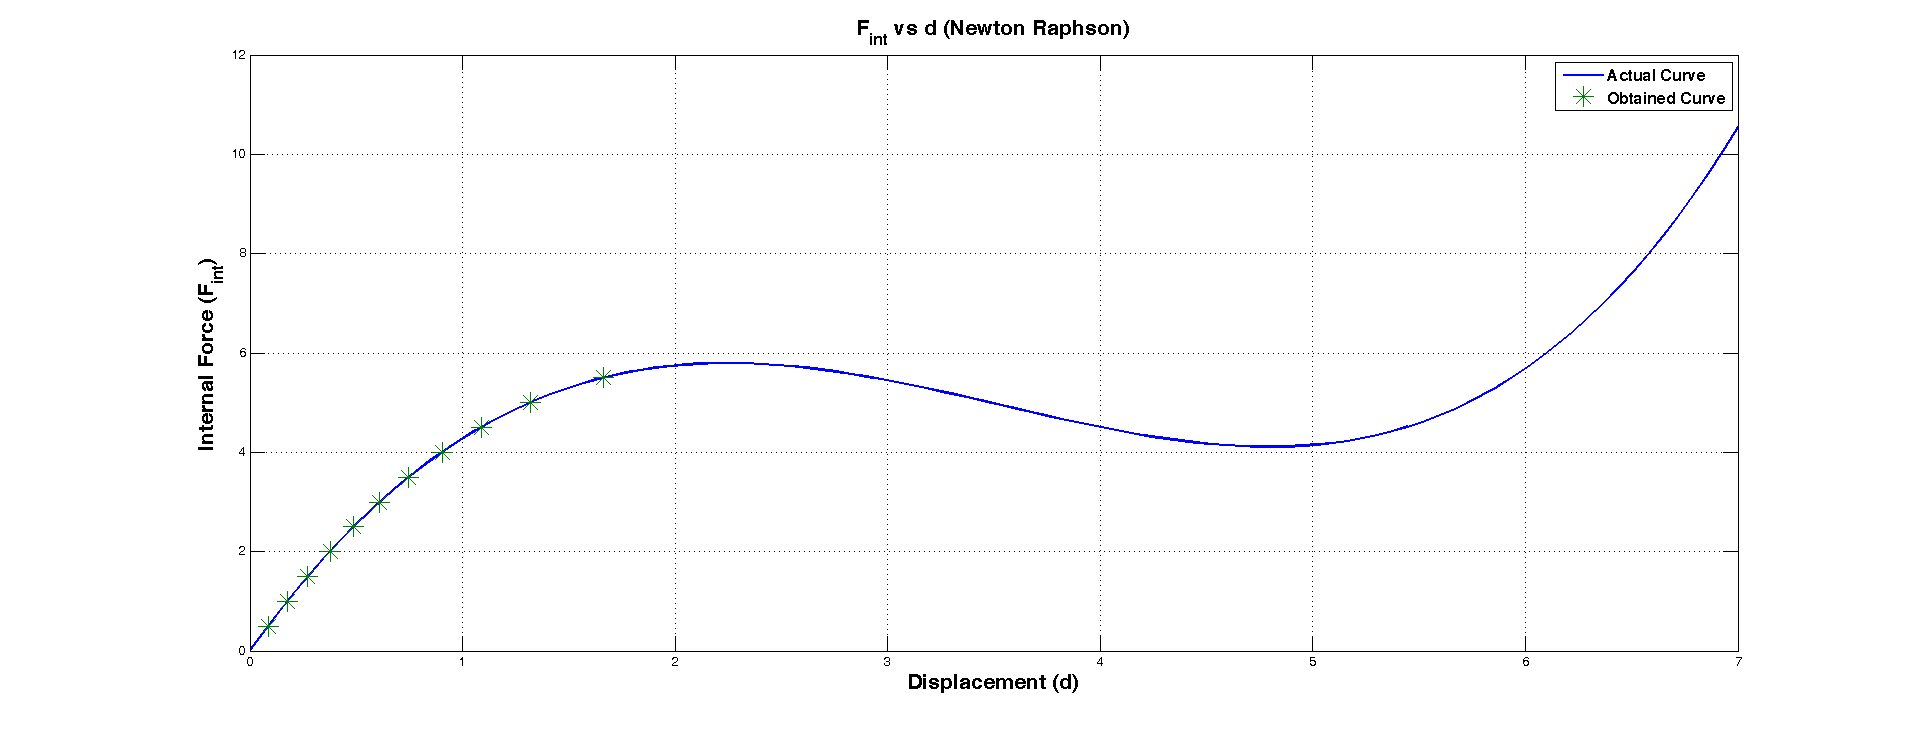
\includegraphics[width=7in]{HW13NR} \nonumber
\end{center}
\begin{center}
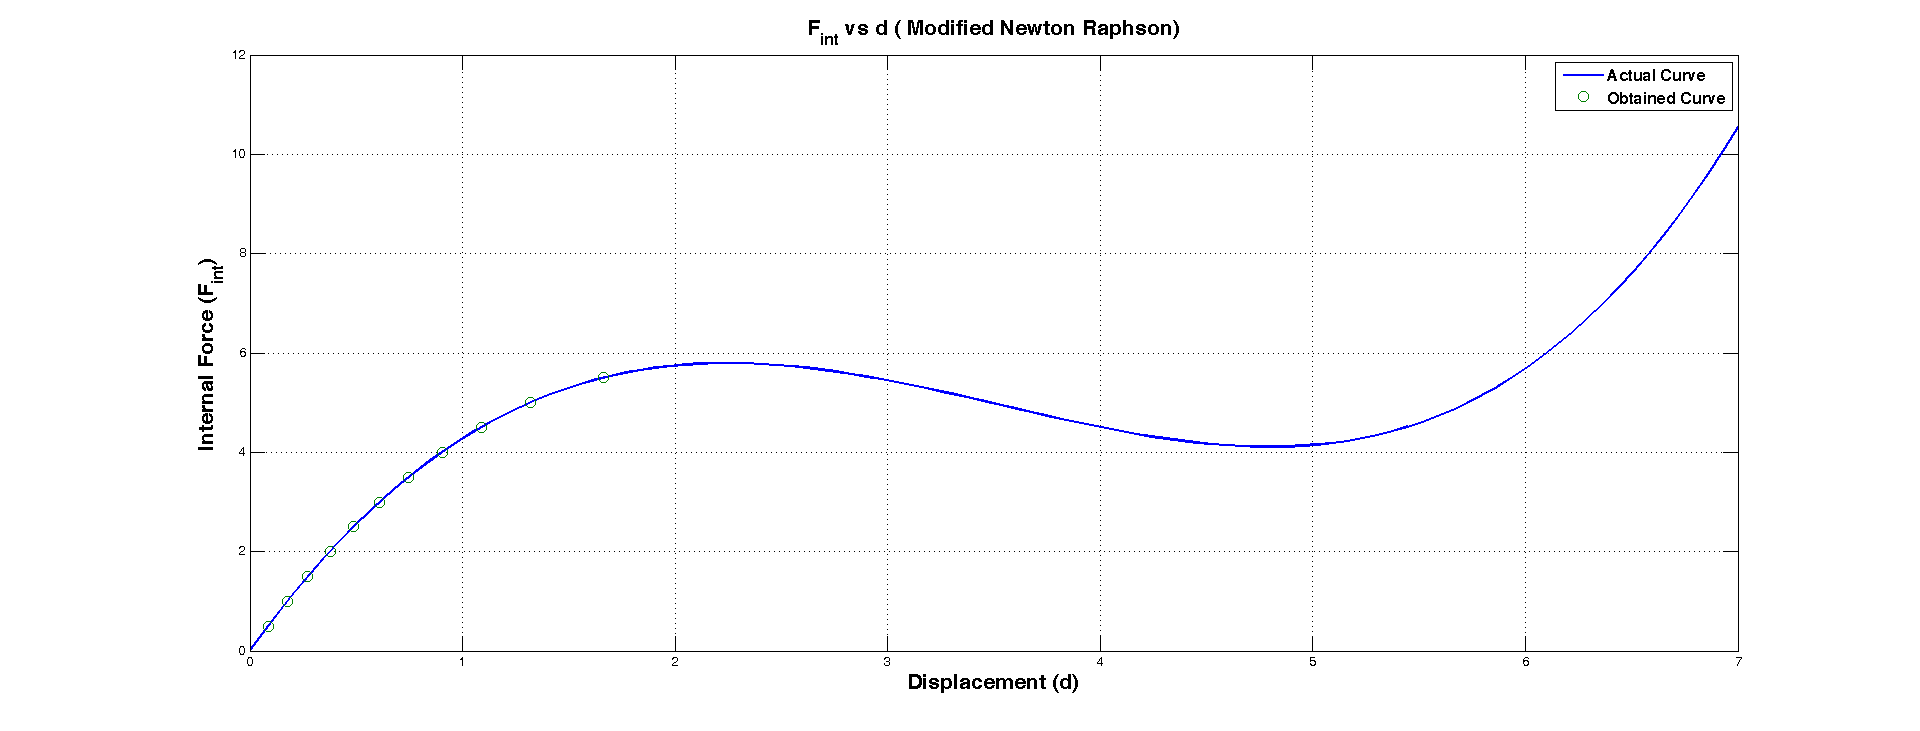
\includegraphics[width=7in]{HW13MNR} \nonumber
\end{center}
\newpage
\subsection*{Residual Reduction: Modified Newton Raphson}
\begin{table}[htbp]
  \centering
  \caption{Residual Reduction in Modified Newton Raphson}
    \begin{tabular}{rrrrrrrrrrrr}
    \toprule
    \multicolumn{1}{l}{\textbf{i}} & \multicolumn{1}{l}{\textbf{Step 1}} & \multicolumn{1}{l}{\textbf{Step 2}} & \multicolumn{1}{l}{\textbf{Step 3}} & \multicolumn{1}{l}{\textbf{Step 4}} & \multicolumn{1}{l}{\textbf{Step 5}} & \multicolumn{1}{l}{\textbf{Step 6}} & \multicolumn{1}{l}{\textbf{Step 7}} & \multicolumn{1}{l}{\textbf{Step 8}} & \multicolumn{1}{l}{\textbf{Step 9}} & \multicolumn{1}{l}{\textbf{Step 10}} & \multicolumn{1}{l}{\textbf{Step 11}} \\
    \midrule
    1     &       &       &       &       &       &       &       &       &       &       &  \\
    2     & 0.012 & 0.013 & 0.015 & 0.016 & 0.018 & 0.02  & 0.023 & 0.028 & 0.033 & 0.0422 & 0.0548 \\
    3     & 6E-04 & 8E-04 & 9E-04 & 0.001 & 0.001 & 0.002 & 0.002 & 0.004 & 0.005 & 0.0094 & 0.0189 \\
    4     & 3E-05 & 4E-05 & 6E-05 & 8E-05 & 1E-04 & 2E-04 & 3E-04 & 5E-04 & 9E-04 & 0.0023 & 0.0075 \\
    5     & 2E-06 & 3E-06 & 4E-06 & 6E-06 & 9E-06 & 2E-05 & 3E-05 & 6E-05 & 2E-04 & 0.0005 & 0.0031 \\
    6     & 1E-07 & 1E-07 & 2E-07 & 4E-07 & 8E-07 & 1E-06 & 3E-06 & 9E-06 & 3E-05 & 0.0001 & 0.0013 \\
    7     & 5E-09 & 9E-09 & 2E-08 & 3E-08 & 6E-08 & 1E-07 & 4E-07 & 1E-06 & 5E-06 & 3E-05 & 0.0006 \\
    8     & 3E-10 & 5E-10 & 1E-09 & 2E-09 & 5E-09 & 1E-08 & 4E-08 & 2E-07 & 8E-07 & 8E-06 & 0.0002 \\
    9     & 1E-11 & 3E-11 & 6E-11 & 2E-10 & 4E-10 & 1E-09 & 4E-09 & 2E-08 & 1E-07 & 2E-06 & 0.0001 \\
    10    & 8E-13 & 2E-12 & 4E-12 & 1E-11 & 3E-11 & 1E-10 & 5E-10 & 3E-09 & 3E-08 & 5E-07 & 4E-05 \\
    11    & 4E-14 & 1E-13 & 3E-13 & 8E-13 & 3E-12 & 1E-11 & 5E-11 & 4E-10 & 4E-09 & 1E-07 & 2E-05 \\
    12    & 2E-15 & 6E-15 & 2E-14 & 6E-14 & 2E-13 & 1E-12 & 6E-12 & 5E-11 & 8E-10 & 3E-08 & 8E-06 \\
    13    & 0     & 0     & 1E-15 & 4E-15 & 2E-14 & 9E-14 & 7E-13 & 7E-12 & 1E-10 & 7E-09 & 3E-06 \\
    14    &       &       & 0     & 0     & 0     & 9E-15 & 7E-14 & 9E-13 & 2E-11 & 2E-09 & 1E-06 \\
    15    &       &       & 0     & 0     & 0     & 0     & 9E-15 & 1E-13 & 4E-12 & 4E-10 & 6E-07 \\
    16    &       &       & 0     & 0     & 0     & 0     & 0     & 2E-14 & 7E-13 & 1E-10 & 3E-07 \\
    17    &       &       & 0     & 0     & 0     & 0     & 0     & 0     & 1E-13 & 3E-11 & 1E-07 \\
    18    &       &       & 0     & 0     & 0     & 0     & 0     & 0     & 2E-14 & 6E-12 & 5E-08 \\
    19    &       &       & 0     & 0     & 0     & 0     & 0     & 0     & 0     & 2E-12 & 2E-08 \\
    20    &       &       & 0     & 0     & 0     & 0     & 0     & 0     & 0     & 4E-13 & 9E-09 \\
    21    &       &       & 0     & 0     & 0     & 0     & 0     & 0     & 0     & 9E-14 & 4E-09 \\
    22    &       &       & 0     & 0     & 0     & 0     & 0     & 0     & 0     & 3E-14 & 2E-09 \\
    23    &       &       & 0     & 0     & 0     & 0     & 0     & 0     & 0     & 0     & 7E-10 \\
    24    &       &       & 0     & 0     & 0     & 0     & 0     & 0     & 0     & 0     & 3E-10 \\
    25    &       &       & 0     & 0     & 0     & 0     & 0     & 0     & 0     & 0     & 1E-10 \\
    26    &       &       & 0     & 0     & 0     & 0     & 0     & 0     & 0     & 0     & 5E-11 \\
    27    &       &       & 0     & 0     & 0     & 0     & 0     & 0     & 0     & 0     & 2E-11 \\
    28    &       &       & 0     & 0     & 0     & 0     & 0     & 0     & 0     & 0     & 1E-11 \\
    29    &       &       & 0     & 0     & 0     & 0     & 0     & 0     & 0     & 0     & 4E-12 \\
    30    &       &       & 0     & 0     & 0     & 0     & 0     & 0     & 0     & 0     & 2E-12 \\
    31    &       &       & 0     & 0     & 0     & 0     & 0     & 0     & 0     & 0     & 7E-13 \\
    32    &       &       & 0     & 0     & 0     & 0     & 0     & 0     & 0     & 0     & 3E-13 \\
    33    &       &       & 0     & 0     & 0     & 0     & 0     & 0     & 0     & 0     & 1E-13 \\
    34    &       &       & 0     & 0     & 0     & 0     & 0     & 0     & 0     & 0     & 6E-14 \\
    \bottomrule
    \end{tabular}%
  \label{tab:addlabel}%
\end{table}%
\subsection*{Residual Reduction: Newton Raphson}
\begin{table}[htbp]
  \centering
  \caption{Residual Reduction in Newton Raphson}
    \begin{tabular}{rrrrrrrrrrrr}
    \toprule
    \multicolumn{1}{l}{\textbf{i}} & \multicolumn{1}{l}{\textbf{Step 1}} & \multicolumn{1}{l}{\textbf{Step 2}} & \multicolumn{1}{l}{\textbf{Step 3}} & \multicolumn{1}{l}{\textbf{Step 4}} & \multicolumn{1}{l}{\textbf{Step 5}} & \multicolumn{1}{l}{\textbf{Step 6}} & \multicolumn{1}{l}{\textbf{Step 7}} & \multicolumn{1}{l}{\textbf{Step 8}} & \multicolumn{1}{l}{\textbf{Step 9}} & \multicolumn{1}{l}{\textbf{Step 10}} & \multicolumn{1}{l}{\textbf{Step 11}} \\
    \midrule
    1     &       &       &       &       &       &       &       &       &       &       &  \\
    2     & 0.013 & 0.014 & 0.016 & 0.017 & 0.02  & 0.022 & 0.026 & 0.032 & 0.04  & 0.0536 & 0.0811 \\
    3     & 1E-05 & 1E-05 & 2E-05 & 2E-05 & 3E-05 & 5E-05 & 9E-05 & 2E-04 & 3E-04 & 0.001 & 0.0054 \\
    4     & 5E-12 & 1E-11 & 2E-11 & 4E-11 & 1E-10 & 3E-10 & 1E-09 & 4E-09 & 3E-08 & 4E-07 & 3E-05 \\
    \bottomrule
    \end{tabular}%
  \label{tab:addlabel}%
\end{table}%
\newpage
\subsection*{Soft Spots and Overall performance}
\begin{itemize}
\item The Newton Raphson Algorithm converges fairly quickly because the stiffness (slope) is updated in each iteration. This is costly but in turn enhances the overall performance of the Algorithm
\item In case of the Modified Newton Raphson Algorithm the stiffness is not updated at every iteration, hence the cost is saved, but it takes many more iterations to converge to a similar tolerance level when compared to the Newton-Raphson Algorithm.
\item Both the algorithms, when used with the incremental load method are unable to capture the fall in the actual force as the slope equals zero at $F = 6$
\item When encountered with unloading (decreasing F) a similar problem could occur as explained in the previous point.
\end{itemize}
\end{document}